% !TEX root = ./tileheat.tex
\section{TileHeat framework}
\label{sec:algorithms}

In this section, we present the TileHeat framework for selecting and caching tiles. We begin with an overview of the framework and the context it is used in (Sections~\ref{sec:tileheat:overview} and~\ref{sec:tileheat:tasks}), followed by two different algorithms for tile ranking (Sections~\ref{sec:heat:hw} and~\ref{sec:heat:d}).   

\vspace{4ex}

\subsection{Overview}
\label{sec:tileheat:overview}
Based on our observations of the workload in Section \ref{sec:analysis}, we have designed the TileHeat framework for a repeated cycle of time periods containing a high- and low-load window. This basic cycle is outlined in Figure~\ref{fig:high:low}.

The life cycle of a system that uses TileHeat to manage tiles is as follows: We organize processing in TileHeat into a sequence of \emph{time periods}. Each time period is composed of two \emph{time windows}: the high-load window and the low-load window. Throughout both windows, the geospatial web service is available for clients and therefore must carry out normal processing of user requests, i.e., \texttt{GET} and \texttt{PUT}. During the low load window, however, we can additionally \emph{select and pre-compute tiles} that we expect to be accessed during the next time window, based on access patterns observed for previous time periods. In the following, we describe how we carry out the selection and pre-computation of tiles.

\begin{figure}
\centering
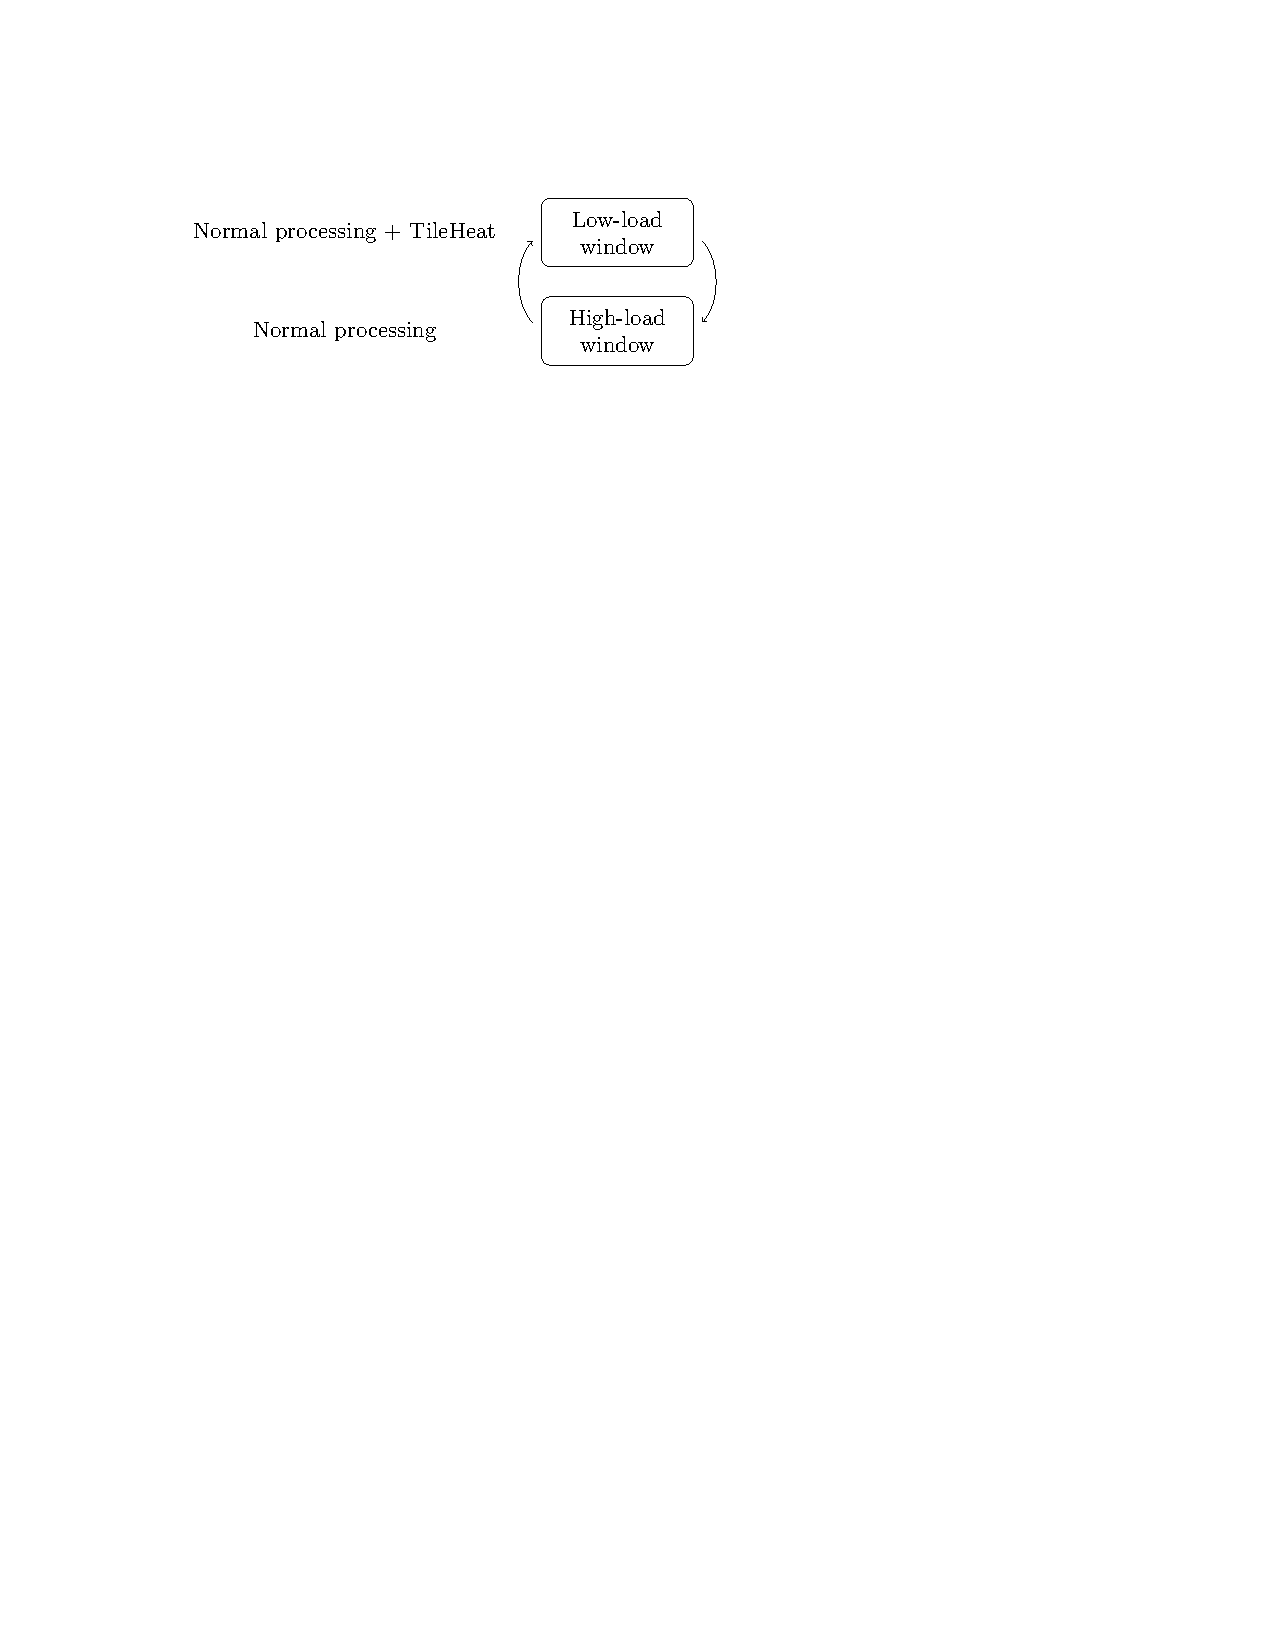
\includegraphics[scale=0.8]{figoverview}
\caption{Time periods and time windows: Processing during high- and low-load windows.}
\label{fig:high:low}
\end{figure}

%We assume that the base data from which the tiles are generated, gets updated frequently, which makes it a bad strategy to compute the entire set of tiles. 

\subsection{Tasks performed by TileHeat}
\label{sec:tileheat:tasks}

TileHeat is a framework for embedding tile selection algorithms into a log analysis procedure. The log analysis procedure computes a set of $n$ heatmaps, and passes these to tile selection. Tile selection in turn employs a \emph{prediction algorithm}, which predicts the heatmap for time $t + 1$. TileHeat uses the predicted heatmap to select which tiles to materialize for the next high-load window. 

The following steps are performed in time period $t+1$ by the TileHeat framework:
%
\begin{enumerate}
\item A prediction algorithm uses heatmaps for time periods $t-n$ to $t$ to predict the heatmap for time period $t+1$.
\item The tiles in the predicted heatmap are sorted in non-increasing order by heat.
\item The $k$ first tiles that are not already materialized are selected.
\item The materialization of the $k$ tiles is scheduled.
\end{enumerate}

The number $k$ is chosen as the number of tiles that can be materialized during the current low-load window. Various algorithms can be used to predict the heatmap for $t + 1$. In this work, we present two algorithms for the TileHeat framework: HEAT-HW (Section~\ref{sec:heat:hw}) and HEAT-D (Section~\ref{sec:heat:d}).

The running time of TileHeat can be estimated as follows. Let $m$ be the number of requests in the request log for time periods $t-n$ to $t$. We assume that the number of \texttt{GET} requests for each log request is bounded by a constant. The number of tile requests is therefore $O(m)$. By using a hash table, we can build the heatmaps in (expected) $O(m)$ time. As the sorting step takes at most $O(m)$ tiles as input, the (expected) running time of TileHeat is $O(m \log m)$ --- plus the running time of the prediction algorithm. 

\subsection{HEAT-HW algorithm}
\label{sec:heat:hw}
We have developed the HEAT-HW algorithm, which uses exponential smoothing applied to the heatmaps for time periods $t-n$ to $t$. Specifically, we use Holt-Winter double exponential smoothing~\cite{chatfield88}, which takes the trend of the observed variable into account. We motivate our choice of smoothing function in two ways:

\begin{enumerate}
\item We apply a smoothing function in general to avoid overfitting to the training data. Although the data we have analyzed is very stable, we introduce smoothing to prepare the algorithm for less stable workloads.
\item We use Holt-Winter smoothing in particular because it captures the trend in popularity for each tile. In future work, we would like to make use of the trend to adapt proactively to sudden rises in popularity for a geographical subregion by increasing the number of nodes serving those tiles. This of course implies a multi-node cache.
\end{enumerate}

Exponential smoothing is applied by treating each heat tile index $(i,j,z)$ as a separate variable. The equations for double exponential smoothing for heatmaps are given below (assuming that the first time period is $0$).

\begin{eqnarray*}
s_{i,j,z}^0 & = & h_{i,j,z}^0 \\
b_{i,j,z}^0 & = & h_{i,j,z}^1 - h_{i,j,z}^0 \\
s_{i,j,z}^{t+1} & = & \alpha h_{i,j,z}^0 + (1 - \alpha)(s_{i,j,z}^{t} + b_{i,j,z}^{t} ) \\
b_{i,j,z}^{t+1} & = & \beta (s_{i,j,z}^{t+1} - s_{i,j,z}^{t}) + (1 - \beta) b_{i,j,z}^{t}  \\
\end{eqnarray*}

As defined in Section~\ref{sec:heatmap:model}, $h_{i,j,z}^t$ is the observed heat of tile $(i,j,z)$ in time period $t$; $s_{i,j,z}^t$ is the smoothed value for time $t$ and $b_{i,j,z}^t$ is the trend for time $t$. Parameters $\alpha$ and $\beta$ are determined experimentally.

\subsection{HEAT-D algorithm}
\label{sec:heat:d}
The exponential smoothing as used in HEAT-HW only ranks tiles that are actually requested in the training data. Often, the training data is sparse, or tiles that are not accessed in the time periods $t-n$ to $t$ get accessed in time $t+1$, due to local changes in the spatial distribution of tile requests. 

HEAT-D is inspired by Tobler's first law of geography: ``Everything is related to everything else, but near things are more related than distant things''. HEAT-D works by applying a dissipation step to all heatmaps prior to applying Holt-Winter double exponential smoothing. The dissipation step is similar to the Jacobi method used for numerically solving the heat equation~\cite{templates}.

The following steps are performed by HEAT-D: 

\begin{enumerate}

\item For each heatmap of time periods $t-n$ to $t$, apply $p$ iterations of the dissipation step. An iteration consists of moving a fraction of the heat of each cell $(i,j,z)$ to its eight neighbors. This fraction is controlled by  a dissipation constant $\mu$. The corresponding differences in heat applied to each cell are shown in Figure~\ref{fig:dissipate}. 

\item Apply HEAT-HW over the heatmaps obtained in the step above. 

\end{enumerate}

%We apply $p$ rounds of the dissipation step to each heatmap in the training data. For each index $(i,j,z)$ in the heatmap, the dissipation step moves a fraction of the heat for that tile to its eight neighbors, based on a dissipation constant $\mu$. The process is illustrated in Figure~\ref{fig:dissipate}.

\begin{figure}
\centering
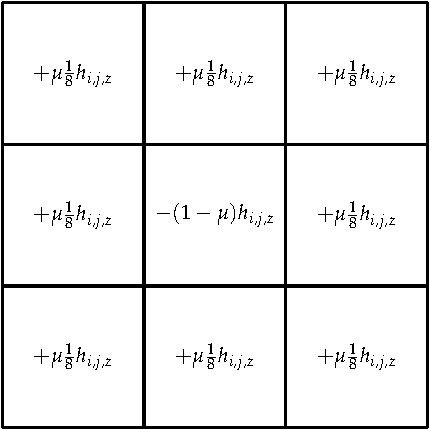
\includegraphics[scale=1]{disspate2}
\caption{Each dissipation step transfers heat from a center cell to each of it's eight neighbors. The center cell $(i,j,z)$ loses $(1 - \mu) h_{i,j,z}$ heat, and the neighbors gain $\mu \frac{1}{8} h_(i,j,z)$ heat. This is repeated for all center cells that are not on the border of the heatmap, using double buffering to avoid prematurely updating the heat of a cell.}
\label{fig:dissipate}
\end{figure}

The result of running dissipation on a sparse sample set can be seen in Figure~\ref{fig:dissipate_before_after}.

\begin{figure*}
\centering
\begin{tabular}{ll}
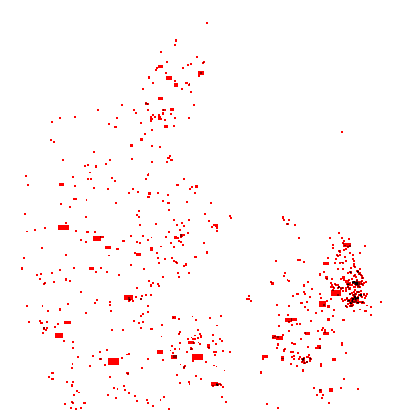
\includegraphics[scale=0.5]{heat_d-before.png} & 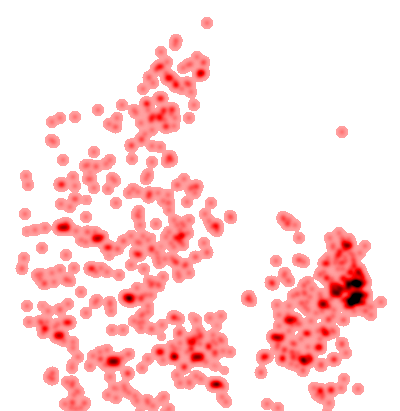
\includegraphics[scale=0.5]{heat_d-after.png} \\
\end{tabular}
\caption{Result of running the dissipation algorithm on a sparse heatmap (left) which contains $1.25\%$ of the samples used to create the heatmaps of Figure~\ref{fig:heatmaps}. The result (right) covers the hot regions of the heatmaps in Figure~\ref{fig:heatmaps} much better.}
\label{fig:dissipate_before_after}
\end{figure*}

 